%% LyX 2.2.4 created this file.  For more info, see http://www.lyx.org/.
%% Do not edit unless you really know what you are doing.
\documentclass[twoside]{bioinfo}
\setcounter{secnumdepth}{3}
\setcounter{tocdepth}{3}
\usepackage{url}
\usepackage{graphicx}
\usepackage[unicode=true]
 {hyperref}

\makeatletter
%%%%%%%%%%%%%%%%%%%%%%%%%%%%%% User specified LaTeX commands.
\copyrightyear{2015} \pubyear{2015}

\access{Advance Access Publication Date: Day Month Year}
\appnotes{Manuscript Category}

\let\cite\citep

\makeatother

\begin{document}
\firstpage{1}

\subtitle{Genetics and population analysis}

\title[short Title]{MultiGWAS: Integrando m�ltiples herramientas para realizar GWAS en tetraploides}

\author[Sample \textit{et~al}.]{Luis Garreta\,$^{\text{\sfb 1,}*}$, Paula Reyes\,$^{\text{\sfb 1}}$ and Ivania Cer�n\,$^{\text{\sfb 1,}*}$}
\address{$^{\text{\sf 1}}$Colombian Agricultural Research Corporation (Agrosavia), Kil�metro 14, V�a a Mosquera, 250047, Colombia}

\corresp{$^\ast$To whom correspondence should be addressed.}

\history{Received on XXXXX; revised on XXXXX; accepted on XXXXX}

\editor{Associate Editor: XXXXXXX}

\twocolumn[
\begin{@twocolumnfalse}

\abstract{\textbf{Motivation:} Text Text Text Text Text Text Text Text Text Text Text Text Text
Text Text Text Text Text Text Text Text Text Text Text Text Text Text Text Text Text Text Text
Text Text Text Text Text Text Text Text Text Text Text Text Text Text Text Text Text Text Text
Text Text Text Text Text Text
Text Text Text Text Text.\\
\textbf{Results:} Text  Text Text Text Text Text Text Text Text Text  Text Text Text Text Text
Text Text Text Text Text Text Text Text Text Text Text Text Text  Text Text Text Text Text Text\\
\textbf{Availability:} Text  Text Text Text Text Text Text Text Text Text  Text Text Text Text
Text Text Text Text Text Text Text Text Text Text Text Text Text Text  Text\\
\textbf{Contact:} \href{name@bio.com}{name@bio.com}\\
\textbf{Supplementary information:} Supplementary data are available at \textit{Bioinformatics}
online.}

\maketitle \end{@twocolumnfalse}]

\begin{figure}[!t]
\noindent\begin{minipage}[b][1\totalheight][t]{1\columnwidth}%
\noindent\begin{minipage}[t]{1\columnwidth}%
Caso 1:%
\end{minipage} 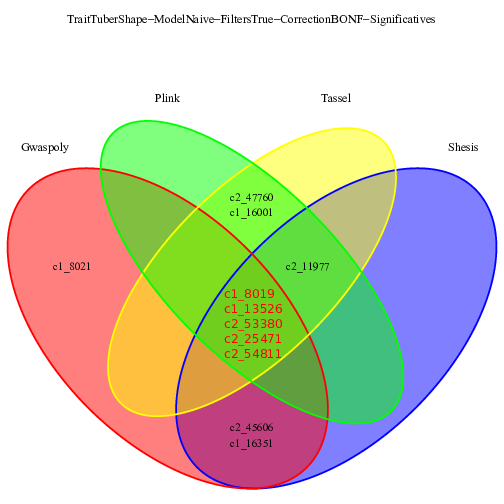
\includegraphics[viewport=5bp 15bp 500bp 410bp,clip,scale=0.43]{/home/lg/agrosavia/development/gwas-polypipeline/paper/old/paper0/results/out-Gwaspoly-Naive-Bonf-Sign}%
\end{minipage}

\noindent\begin{minipage}[t]{1\columnwidth}%
\noindent\begin{minipage}[t]{1\columnwidth}%
Caso 2:%
\end{minipage} 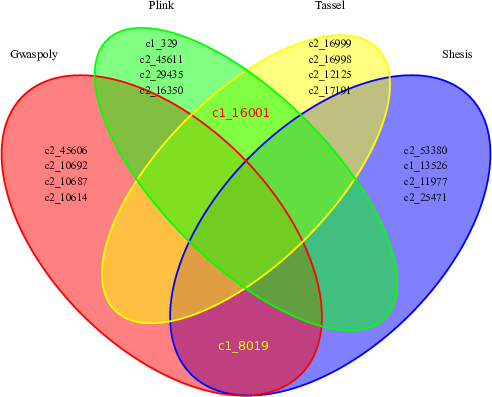
\includegraphics[viewport=5bp 15bp 500bp 410bp,clip,scale=0.43]{/home/lg/agrosavia/development/gwas-polypipeline/paper/old/paper0/results/out-Gwaspoly-Structure-Bonf-Best5}%
\end{minipage}

\noindent\begin{minipage}[t]{1\columnwidth}%
\noindent\begin{minipage}[t]{1\columnwidth}%
Caso 3:%
\end{minipage} 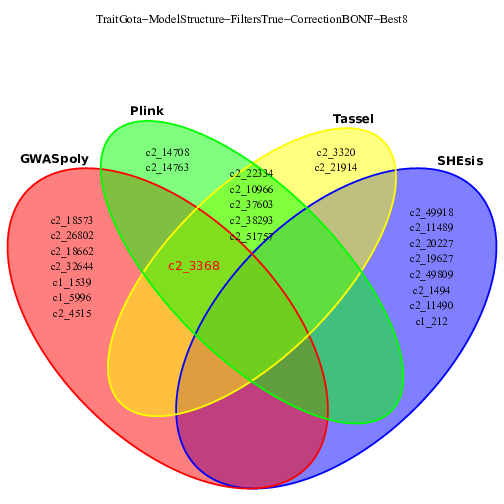
\includegraphics[viewport=5bp 15bp 500bp 400bp,clip,scale=0.43]{/home/lg/agrosavia/development/gwas-polypipeline/paper/old/paper0/results/out-Gota-Structure-BONF-Best8}%
\end{minipage}

\caption{MultiGwasTool aplicado en tres rasgos de poblaciones de papa. En rojo
los marcadores com�nes. Caso1: las cuatro herramientas encuentran
marcadores comunes. Caso 2: Las dos herramientas diploides encuentran
un marcador com�n, mientras que las dos poliploides encuentran un
marcador com�n diferente. Caso 3: Tres de las cuatro herramientas
encuentran marcadores comunes.\label{fig:Cases}}
\end{figure}


\section{M�todos }

El control de calidad de los datos se lleva a cabo a trav�s de filtros
que se aplican tanto al genotipo y al fenotipo y que buscan eliminar
individuos y marcadores que no cumplan ciertos criterios y que pueden
sesgar el an�lisis. Algunos filtros se aplican por defecto, como la
eliminaci�n de duplicados (tanto de individuos como de marcadores)
y la eliminaci�n de individuos sin informaci�n genot�pica. Otros filtros
se pueden seleccionar o ajustar sus valores a trav�s del archivo de
configuraci�n, entre estos: frecuencia del alelo menor, porcentaje
de individuos/marcadores con perdida de informaci�n, y marcadores
en equilibrio de Hardy-Weinber.

MultiGWAS ejecuta GWAS usando dos modelos estad�sticos de los cuatro
propuestos por Sharma et al.: modelo Naive y modelo Completo\footnote{Excepto la herramienta SHEsis que solo soporta el modelo Naive.}\nocite{Sharma2018}.
El modelo Naive no realiza correcci�n de estructura poblacional ni
considera las relaciones de parentesco; mientras que el moodelo Completo
realiza la correcci�n de estructura poblacional mediante el c�lculo
de los 10 primeros componentes principales que se ajustan como efectos
fijos en cada herramienta; y las relaciones de parentesco entre individuos
que se ajustan de acuerdo al algoritmo utilizado por defecto en cada
herramienta. GWASpoly calcula el parentesco mediante la matriz K
como $MM^T$, donde \emph{M} es la matriz de genotipos centrada (individuos
x marcadores) \cite{Rosyara2016}; en Plink, primero se calculan los
individuos relacionados mediante el algoritmo KING-Robust implementado
en la herramienta king \cite{Manichaikul2010} y luego se los remueve
de los datos del genotipo; y Tassel que calcula el parentesco mediante
el m�todo Centered-Identity by State (Centered-IBS) de Endelman and
Jannink \cite{Endelman2012}. 

\section{Implementaci�n}

MultiGWAS est� implementado en R como una aplicaci�n que se ejecuta
en l�nea de comandos, ya sea en una terminal en ambiente Linux o Mac.
La entrada consiste en un �nico archivo de configuraci�n donde se
especifica los nombres de los archivos de entrada (genotipo y fenotipo),
el modelo de GWAS a ejecutar (Naive o Completo), y la especificaci�n
de los valores de los distintos filtros para aplicar en el genotipo
y fenotipo.

MultiGWAS integra cuatro herramientas de GWAS que deben estar previamente
instaladas. Esto se puede llevar ya sea de forma autom�tica, a trav�s
de la ejecuci�n de un script propio de configuraci�n que acompa�a
a MultiGWAS; o de forma manual, seguiendo las instrucciones de instalaci�n
propias de cada herramienta: GWASPoly (\href{https://potatobreeding.cals.wisc.edu/software}{https://potatobreeding.cals.wisc.edu/software});
Plink utiliza tres programas binarios: plink1.9 (\href{https://www.cog-genomics.org/plink}{https://www.cog-genomics.org/plink}),
 plink2.0 \href{https://www.cog-genomics.org/plink/2.0)}{https://www.cog-genomics.org/plink/2.0)},
y king (\url{http://people.virginia.edu/~wc9c/KING}). Tassel (\href{https://www.maizegenetics.net/tassel}{https://www.maizegenetics.net/tassel}),

\section{Resultados and Discussion}

En la figura \ref{fig:Cases} se muestran tres resultados producidos
por MultiGWAS al ejecutarse sobre dos conjuntos de datos: el genotipo
y fenotipo recolectados como parte del proyecto Solanaceae Coordinated
Agricultural Project (SolCAP) y usados para probar el software de
GWASpoly \cite{Rosyara2016}; y el genotipo y fenotipo recolectados
en el estudio de la Colecci�n Central Colombiana de Papa (CCC) \cite{Berdugo-Cely2017}. 

En el primer caso, figura \ref{fig:Cases}.A, las cuatro herramientas
coinciden en un conjunto grande de marcadores significativos, ya que
el modelo GWAS aplicado fue Naive, sin ning�n control de estructura
poblacional ni consideraci�n de relaciones de parentesco, y con la
posibilidad de encontrar asociaciones falsas. Entre esos marcadores
comunes, el primero de la lista y de mayor puntaje es el c1\_8019,
reportado por Rosyara et al. \cite{Rosyara2016} como rasgo cuantitativo
m�s significante. En el segundo caso, figura \ref{fig:Cases}.B, se
ejecut� MultiGWAS sobre el mismo conjunto de datos pero ahora con
el modelo Completo de GWAS, el cual filtra los posibles falsos negativos
reduciendo el n�mero de marcadores comunes a dos, c1\_16001 y c1\_8019,
el primero encontrado como m�s significativo solo por las herramientas
diploides (Plink y Tasse), y el segundo encontrado solo para las herramientas
poliploides (GWASpoly y SHEsis). Este �ltimo es el mismo marcador
c1\_8019 encontrado por las cuatro herramientas en el caso anterior.
El tercer caso, figura \ref{fig:Cases}.C, el an�lisis se realiz�
sobre el conjunto de datos de la CCC (ver m�todos) y muestra como
tres de las cuatro herramientas encuentran un marcador com�n. En este
caso el modelo utilizado fue el Completo, que lo soportan estas tres
herramientas y que permite filtrar falsas asociaciones. Sin embargo,
la herramienta SHEsis soporta solo el modelo Naive, sin control de
los posibles falsos positivos y por lo tanto con resultados muy diferentes
a los de las otras herramientas.

\bibliographystyle{natbib}
\bibliography{multiGWAS}

\end{document}
